\mysection{Division du travail}
Pour faire le travail un peu plus simple en concentrant les efforts en petits tâches chacune par foi, optimisant le temps. Le travail était divisé en plusieurs \textit{Work Packages}, caqu'un composé par petits tâches. La division et ses respectives tâches peuvent être vu dans les sections \ref{Première Partie  - Lecture} à \ref{Cinquième Partie - Rédaction} suivantes.

\mysubsection{Première Partie  - Lecture}
La première partie consistait en lire le article de WAN Yidong \cite{yidong}, qu'explique d'une façon un peu simplifié le problème et montre des façons de calculer les gains entre la tension des bus et la puissance reactive des charges, en utilisant scripts écrits en \gls{DPL} dans le logiciel PowerFactory et la création d'une matrix de gain.

Après la lecture du article, la lecture de quelques parties de la thèse de Marjorie Cosson \cite{cosson:tel-01374469} a fin de comprendre le problème un peu meilleur   proposé et les résultats trouvés. 

Autres lectures supplémentaires ont été faites, \cite{farina2015model} et \cite{mariani2013controllo}. Ces articles utilisent le même réseaux que \cite{cosson:tel-01374469} et quelques données ont aidé pour la reconstruction du réseaux dans le PowerFactory.


\mysubsection{Deuxième Partie - Mise en Main}
Après la lecture des documents commençait l'étude et pris en main du logiciel DIgSILENT PowerFactory, en lisant et regardant les tutoriels a l'internet, en faisant quelques petits exemples du logiciel a fin d'apprendre les outils nécessaires pour faire les tests proposés et après, faire la montage de la modèle du réseaux dans le PowerFactory, le diagramme montré dans la figure \ref{fig:Diagramme_du_reseaux}. 

\mysubsection{Troisième Partie - Programmation}
Pendant ce partie diverses scripts ont été crées en utilisant les langages MATLAB et Python:
\begin{itemize}
	\item Pour charger les valeurs de puissance des charges.
	\item Pour charger les valeurs de puissance des générateurs.
	\item Pour calculer les gains entre les bus et les générateurs.
	\item Pour faire des matrices de gains.
	\item Pour créer des événements de charges et générateurs, faire des simulations et prendre les résultats en graphiques.
\end{itemize}

\mysubsection{Quatrième Partie - Intégration}
	Pendant la quatrième partie la interface entre le PowerFactory et MATLAB a été requise a fin de créer une modèle de régulateur au simulink et utiliser dans le PowerFactory. \doing{ Le Régulateur a été déjà crée et quelques configurations dans le PowerFactory sont manquantes.}
\pagebreak

\mysubsection{Cinquième Partie - Rédaction}
La cinquième partie consistait en élaborer des rapports et autres documents de description du projet, comme ce document par exemple.

\begin{figure}[H]
	\begin{center}	
		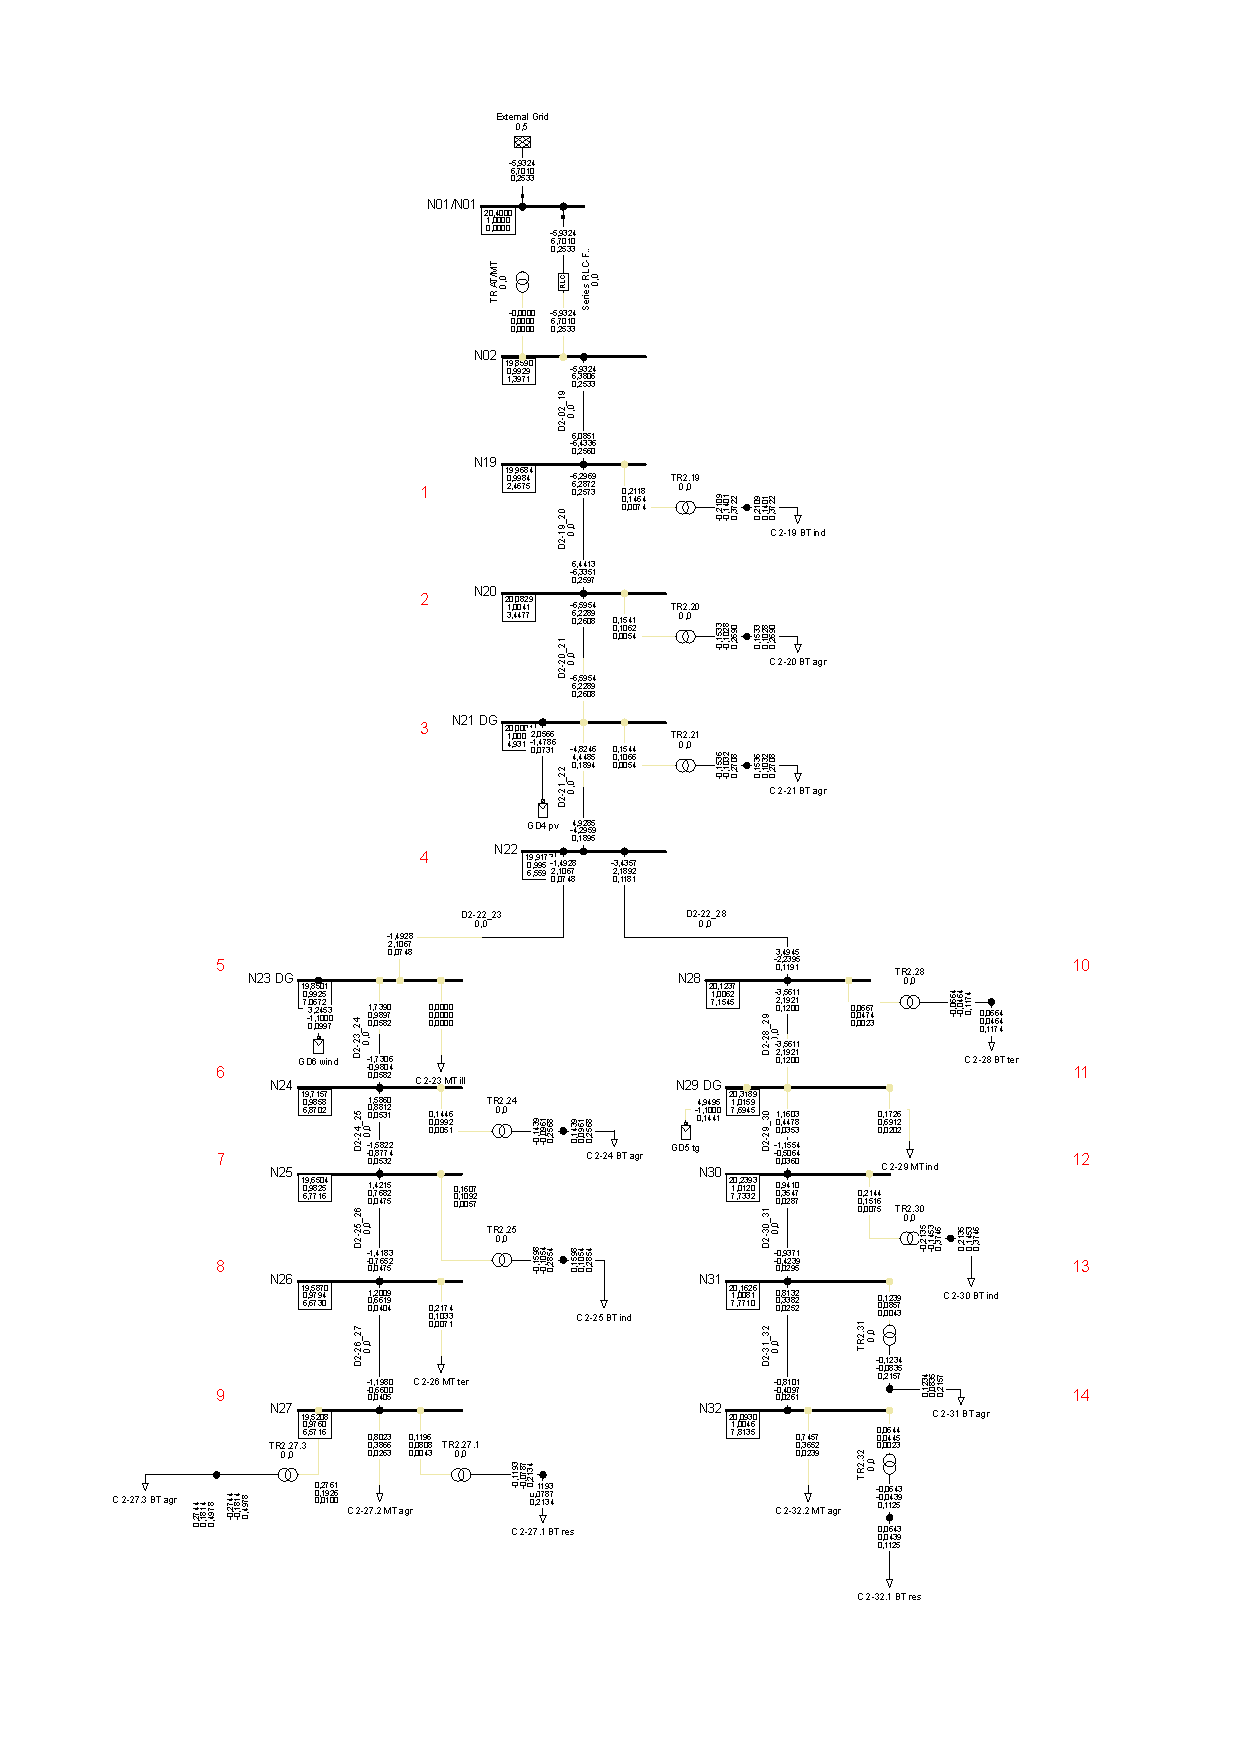
\includegraphics[width=\textwidth]{Division_du_travail/Diagramme_du_reseaux.pdf}
		\caption{Diagramme du reseaux}
		\label{fig:Diagramme_du_reseaux}
	\end{center}
\end{figure}
\newpage